%\section{Metodología}
\justify
\noindent\begin{minipage}[H]{0.53\textwidth}
En esta sección explicaremos la metodología propuesta, en la que detallaremos los pasos del marco de desarrollo del algoritmo, así como los distintos operadores evolutivos.\\

\subsection{Funcionamiento general del algoritmo}


La \hyperref[fig:1]{\textit{figura 1}} muestra el diagrama de flujo general del algoritmo, ajustándose a un esquema típico de algoritmo evolutivo. De manera superficial, el algoritmo recibe las funciones objetivo, el espacio de búsqueda y una serie de parámetros que intervienen en el algoritmo (detallados más adelante), lleva a cabo una primera etapa de inicialización de la población, los vectores de pesos y vecindad de los subproblemas, así como el punto de referencia . A partir de ahí se lleva a cabo un proceso iterativo, en el que se va actualizando la población así como el punto de referencia. De forma que al fin del proceso la población constituye la aproximación del algoritmo al frente de Pareto para el problema tratado.\\


\subsection{Datos de entrada}

El algoritmo recibe como datos de entrada:\\
\begin{itemize}
    \item \textbf{Funciones objetivo}: Un conjunto ordenado de funciones $f_1, \dots, f_m$  consideradas como las funciones objetivo a optimizar por el algoritmo, tratando todas ellas como caso de minimización.\\
    
     \item \textbf{El espacio de búsqueda $\Omega$}: Dado por el producto cartesiano de los espacios de búsqueda de cada una de las variables, acotados superior e inferiormente por $x_{Lj}$ y $x_{Uj}$ respectivamente.\\
     
\end{itemize}
\end{minipage}\hfill\begin{minipage}[H]{0.4\textwidth}
    \begin{figure}[H]
    \centering
    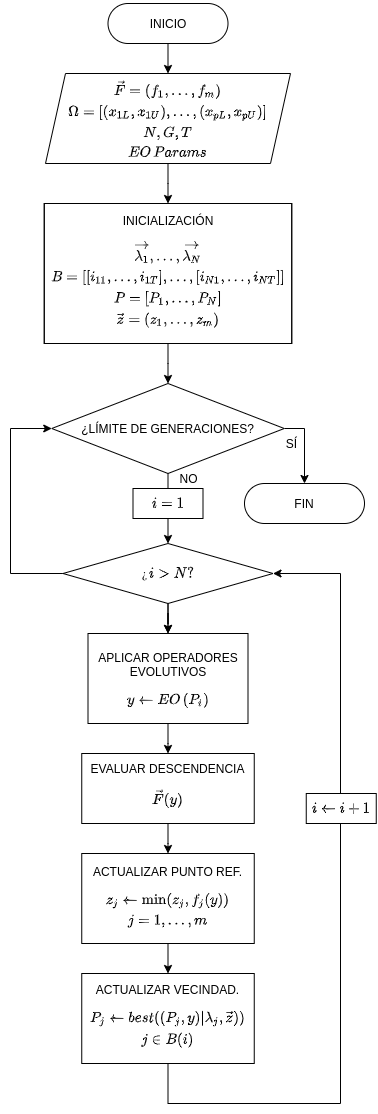
\includegraphics[scale=0.4]{figures/flowchart.png}\\
    \caption{\centering Flujo general del algoritmo}
    \label{fig:1}
\end{figure}
\end{minipage}\\

\begin{itemize}

	\item \textbf{$N$}: Corresponde al número de subproblemas considerados para la división del objetivo mútiple en subobjetivos individuales (por agregación).\\
	
	\item \textbf{$G$}: Corresponde al número de generaciones máximo que realizará el algoritmo, estableciendo un criterio de parada para el mismo.\\
	  
    \item \textbf{$T$}: Corresponde al número de vecinos de cada subproblema esto es, el número de subproblemas, incluyéndose a sí mismo, que serán considerados parte de la vecindad de cada uno de los subproblemas y que influirán en el proceso evolutivo de la población.\\
    
	\item \textbf{Operador evolutivo}: Durante el desarrollo del algoritmo son utilizados operadores de cruce y mutación que han de ser dados por el usuario y que obtendrán un solo individuo como descendiente de cada uno de los individuos de la población.\\
    
	\item \textbf{Otros parámetros}, que detallamos y justificamos en el apartado correspondiente.\\
\end{itemize}

\subsection{Inicialización del algoritmo}

Para poder llevar a cabo la ejecución del algoritmo (proceso iterativo) hemos de disponer de algunos elementos que debemos inicializar al comienzo del algoritmo como son: \\

\begin{itemize}
    \item \textbf{El conjunto de vectores de pesos $\boldsymbol{\lambda_1}, \dots, \boldsymbol{\lambda_N}$}, vectores $m$-dimensionales que identifican a cada subproblema, de forma que para todos ellos debe cumplirse $||\boldsymbol{\lambda_{i}}||_{1} = 1$ y además deben estar distribuidos uniformemente (equiespaciados, tomando como distancia la forma euclídea). Para el caso bi-objetivo, dado que los vectores han de estar normalizados, los $N$ vectores pueden inicializarse siguiendo la expresión $\boldsymbol{\lambda_i} = \left(\frac{i-1}{N-1}, \frac{N-i}{N-1} \right)$ con $i \in \{1, \dots, N\}$.\\
    
    \item \textbf{Vecindad $B(i)$ de cada vector peso $\boldsymbol{\lambda_i}$}, que corresponde al conjunto de los  los $T$ vectores más cercanos a $\boldsymbol{\lambda_i}$ de entre todos los vectores de pesos (incluyendo al propio $\boldsymbol{\lambda_i}$). Nótese que $B(i)$ será considerado el entorno del subproblema $i$, de manera que debe considerarse un entorno cercano ($T$ pequeño) para la evolución del individuo asociado al subproblema considerado.\\

    
    \item \textbf{Inicialización de la población $P$}, con $N$ individuos cada uno de ellos asociados a uno de los subproblemas. Para la inicialización se generará una población aleatoria (respetando los espacios de búsqueda para cada variable). \\

    \item \textbf{Inicialización del punto de referencia $\boldsymbol{z}$}. Recuérdese que según la formulación de Tchebycheff $\boldsymbol{z}^{*}$ debe contener los óptimos globales de cada una de las funciones objetivo en el espacio de búsqueda, pero esto implica resolver $m$ problemas de optimización mono-objetivo. En vez de eso relajaremos $\boldsymbol{z^{*}}$ en $\boldsymbol{z}$ de forma que contendrá en cada momento el mejor (menor) valor para cada $f_j$ ($j = 1, \dots, m$) alcanzado por cualquiera de los individuos evaluados hasta ese instante. De forma que dicho punto de referencia $\boldsymbol{z}$ se irá actualizando de forma síncrona al avance del algoritmo.\\
    
    \item \textbf{Inicialización del conjunto de soluciones no dominadas}. Opcionalmente, el algoritmo puede mantener un conjunto con las soluciones no dominadas por ninguna otra encontrada hasta el momento de forma que el conjunto será actualizado a lo largo del proceso evolutivo.\\
\end{itemize}

\subsection{Desarrollo iterativo}

Tras la inicialización, comienza un proceso iterativo (evolutivo) en el que la población, se actualiza por medio del uso de operadores evolutivos que presentaremos a continuación. Como criterio de parada para este proceso iterativo se tomará el límite de generaciones fijado por el usuario (al igual que en otros algoritmos de carácter evolutivo o inteligencia colectiva se pueden fijar otros criterios de parada anticipada). De manera que para cada iteración (generación) se llevan a cabo las siguientes operaciones:\\

\begin{enumerate}
    \item \textit{Reproducción}: Para cada uno de los individuos se aplican operadores evolutivos (cruce y mutación) de forma que cada individuo es perturbado (en mayor o menor medida) por el entorno. Como entorno se considera el vecindario $B(i)$, del que son tomados, con cierta aleatoriedad, (según el operador) una serie de individuos con los que se aplican los operadores evolutivos. Como el vecindario son los considerados problemas cercanos, es esperable que los cambios entre ellos van a se pequeños por lo que los individuos tenderán a ser parecidos.\\
    
    En concreto se van a implementar y realizar pruebas utilizando los siguientes operadores evolutivos:\\

    \begin{itemize}
        \item  \textbf{EOP1} Basado en \cite{Li2014} y en el propuesto en el enunciado. Se propone es uso de DE (\textit{Diferential Evolution}) + GP (\textit{Gaussian Perturbation}), de manera que, en primer lugar para  el individuo $\boldsymbol{P_i}$ se genera el vector mutante $\boldsymbol{\hat{y}}$, con el uso de cinco vectores `noisy', mediante la expresión:  $$\boldsymbol{\hat{y}}=\boldsymbol{x}^{(r1)} + F \cdot (\boldsymbol{x}^{(r2)}- \boldsymbol{x}^{(r3)}) + rand \cdot  F \cdot (\boldsymbol{x}^{(r4)}- \boldsymbol{x}^{(r5)}) $$
        
        donde $F$ es elegido aleatoriamente de un pool de valores (entre $0$ Y $1$) y $rand$ corresponde a un número aleatorio (entre $0$ y $1$) . Tras esto, se realiza una recombinación utilizando el cruce típico de evolución diferencial, tal que cada componente del vector $\boldsymbol{y}$ se elige aleatoriamente entre $\boldsymbol{\hat{y}}$  y $\boldsymbol{P_i}$, de forma que $\boldsymbol{y}$ contenga al menos una componente del vector mutante. Para ello se sigue la expresión: $$ y_j = \left\lbrace \begin{array}{cl}
            \hat{y}_{ij} & \textrm{si } rand \leq \textit{CR} \textrm{ o } j = \delta\\
             P_{ij} & e.o.c.
        \end{array} \right. $$
        
        donde \textit{CR} corresponde a un parámetro ajustable (entre $0$ y $1$) que representa la probabilidad de cruce, $\delta$ corresponde a una de las componentes del descendiente elegida aleatoriamente y $rand$ corresponde a un número aleatorio (entre $0$ y $1$).\\
        
        Finalmente cada componente de $\boldsymbol{y}$ es perturbada con probabilidad $p_m$ (parámetro ajustable entre $0$ y $1$, típicamente establecida en la literatura como $1/p$, con $p$ la dimensionalidad del espacio de búsqueda) mediante una distribución gaussiana ($N(0,\sigma_{j} = \frac{x_{Uj} - x_{Lj}}{SIG})$ con $SIG$ un parámetro ajustable) . Si alguna de las componentes quedara fuera del espacio de búsqueda correspondiente su valor es establecido al valor de la cota correspondiente.\\
        
        \item \textbf{EOP2}, basado en \cite{Li2009} y \cite{Li2014}, se propone una aproximación con el uso de DE + SBX, de forma que se genera el vector mutante con 5 vectores `noisy' siguiendo la expresión: $$ \boldsymbol{\hat{y}}=\boldsymbol{x}^{(r1)} + F \cdot (\boldsymbol{x}^{(r2)}-\boldsymbol{x}^{(r3)}) + rand \cdot (\boldsymbol{x}^{(r4)}-\boldsymbol{x}^{(r5)})$$ donde  $F$ corresponde a un parámetro de ajuste (fijo) y $rand$ corresponde a un número aleatorio (en $[0,1]$). Una vez ejecutada dicha mutación, el operador de cruce corresponde al mismo que EOP1. El vector resultante $\boldsymbol{y}$ es finalmente perturbado en cada componente utilizando la expresión (proveniente de SBX) siguiendo la expresión : $$ y_j = \left\lbrace \begin{array}{ll}
            y_j + \sigma_{k} \cdot (x_{Uj}-y_{Lj}) & \textit{si } rand < p_{m} \\
            y_j & e.o.c
        \end{array} \right., \sigma_k = \left\lbrace \begin{array}{ll}
            (2 \cdot rand)^{\frac{1}{\eta+1}}-1 & \textit{si } rand < 0.5 \\
            1 - (2 - 2 \cdot rand)^{\frac{1}{\eta+1}} & e.o.c
        \end{array} \right.$$ 
        donde $rand$ corresponde a un número aleatorio (entre $0$ y $1$), distinto en cada expresión (izqda. y dcha.), $\eta$ corresponde al índice de distribución de cruce\footnote{El valor numérico de este parámetro de control es inversamente proporcional a la cantidad de perturbación en las variables de diseño. Cuanto menor sea el valor de este parámetro de control, mayor será la perturbación y viceversa. Por tanto, un valor más pequeño mejora la resistencia a la convergencia prematura a costa de una búsqueda muy centrada.} y $p_{m}$ la probabilidad de mutación. Finalmente, si alguna componente de $\boldsymbol{y}$ se encuentra fuera de las cotas establecidas para la variable,  es ajustada a la cota correspondiente.\\
        
        \item \textbf{EOP3}, basado en el esquema de Recombinación Uniforme (\textit{Uniform Crossing} (UX)) se propone una aproximación con el uso de UX + GP, de forma que para el individuo $\boldsymbol{P_{i}}$ se genera descendiente $\boldsymbol{y}$, con $\varepsilon \leq T$ vectores tomados aleatoriamente del vecindario, de manera que cada componente del vector mutante es elegida aleatoriamente entre los vectores del entorno: $$ y_j = x^{(ri)}_{j}$$ donde $ri \in B(i)$. Sobre el descendiente se lleva a cabo una mutación (perturbación) gaussiana análoga a la planteada en EOP1. Finalmente, si alguna componente de $\boldsymbol{y}$ se encuentra fuera de las cotas establecidas para la variable,  es ajustada a la cota correspondiente.\\
    \end{itemize}

    \item[2.] \textit{Evaluación}: El descendiente obtenido es evaluado respecto a todos los objetivos $\boldsymbol{F}(\boldsymbol{y})$. Nótese que hemos exigido que el operador evolutivo considerado genere un único descendiente. Aunque en la literatura existen versiones de \textit{MOEA/D} que trabajan con varios descendientes, es muy común encontrar la versión adoptada, con la ventaja de que para cada individuo y cada generación se realiza una única evaluación. \\
    
    \item[3.] \textit{Actualización del punto de referencia $\boldsymbol{z}$}: Recuérdese que $z$ correspondía al vector $m$-dimensional ($m$ el número de objetivos) cuyas componenetes correspondientes correspondían a los pseudo-óptimos (mejores valores obtenidos hasta el momento) luego hemos de actualizar $z$ en aquellas componentes tal que $F_j(\boldsymbol{y}) < z_j$ (con $j=1,\dots,m$).\\
    
    \item[4.] \textit{Actualización del entorno $B(i)$}: Recuérdese que $z$ correspondía al vector $m$-dimensional ($m$ el número de objetivos) cuyas componenetes correspondientes correspondían a los pseudo-óptimos (mejores valores obtenidos hasta el momento) luego hemos de actualizar $z$ en aquellas componentes tal que $F_j(\boldsymbol{y}) < z_j$ (con $j=1,\dots,m$).\\

      \item[5.] \textbf{Actualización del conjunto de soluciones no dominadas}. En caso de que se utilice, se ha de actualizar el conjunto de soluciones no dominadas. De forma que si y sólo si ninguna de las soluciones del conjunto dominan a la valoración del descendiente $\boldsymbol{F}(\boldsymbol{y})$ entonces este pasa a formar parte de las soluciones no dominadas y son eliminadas del conjunto aquellas que son dominadas por $\boldsymbol{F}(\boldsymbol{y})$. En otro caso no se realiza actualización alguna. \\
\end{enumerate}

\subsubsection{Algunas consideraciones}

Dado el proceso iterativo propuesto, aunque no ha sido especificado, el proceso de actualización de la población (y sus valoraciones) se realiza directamente sobre la población, y no se espera para ser efectiva al fin de la generación. Por ello es conveniente que a la hora de llevar a cabo las actualizaciones los elementos se recorran en un orden aleatorio, para tratar de evitar descompensaciones entre los individuos.\\

Además hemos de tener en cuenta que el hecho de realizar la sustitución en los vecinos puede conllevar una alta disminución de la diversidad y llevar al proceso a una convergencia prematura. Por ello, opcionalmente, se puede establecer un parámetro $UN$ (\textit{updations number}) que limite el número de vecinos sustituidos \cite{FranciscoV2010}.\\


\subsection{Final del algoritmo}

\justify

El proceso iterativo previo se realiza hasta alcanzar el criterio de parada, dado por el número máximo de generaciones $G$. De forma que al final del proceso en la última población se tienen justamente los mejores individuos encontrados durante el proceso para cada uno de los subproblemas y cuyas valoraciones constituyen, precisamente, la aproximación al frente de Pareto. \\

En el caso de hacer uso del conjunto de soluciones no dominadas $NSD$ éste sería una aproximación más cercana y más amplia al frente real Pareto-óptimo, dado que en él se encontrarán todas aquellas soluciones no dominadas por ninguna otra de las encontradas durante todo el proceso de búsqueda.\\ 


